Per il training del modello si è utilizzato un dataset pubblico rilasciato da Kaggle\footnote{\url{https://www.kaggle.com/datasets/pavelbiz/eyes-rtte}} contenente 5 mila immagini di sole pupille umane, comodo per il raggiungimento del nostro obiettivo di pupil detection.

Questa volta, per ottenere i file \textit{*.xml} di ogni immagine, abbiamo usufruito di un tool grafico chiamato \textbf{LabelImage}, scaricabile gratuitamente su Github\footnote{\url{https://github.com/tzutalin/labelImg}}. Questo tool ci permetteva di costruire i boxes attorno alla pupilla ottenendo in output per ogni immagine un file \textit{*.xml} contenente le informazioni necessarie: come il nome dell'oggetto su cui si è costruito attorno il box ("pupil"), e le relative coordinate geografiche dei 4 punti del box (xmin, ymin, xmax, ymax).

Prima dell'addestramento della rete era però necessario, usando questi nuovi dati \textit{*.xml}, generare i \textbf{TFRecord}, utili per TensorFlow.
Inoltre, per la corretta generazione dei \textbf{TFRecord}, si è reso necessario compilare il file \textit{labelmap.pbtxt} con al suo interno i nomi e gli id dei nostri oggetti da riconoscere: nel nostro caso un solo item di id pari a 1 e con nome "pupil".

\begin{figure}[htbp]
    \centering
    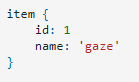
\includegraphics[scale=1]{ReteNeurale/PupilDetection/Dataset/Images/pupillabelmap_item.png}
    \caption{Pupil Detection labelmap.pbtxt}
    \label{fig:pupillabelmap}
\end{figure}
